\section{Iteration 8: Decomposition of the Notification Unit}
\label{add:it8}

\subsection{Step 1: Identify candidate drivers}
\label{add:it8/drivers}

\npar There is only very little functionality delegated to this unit, namely two
cases, UC9 (Notify Customer) and UCx (retrieve customer from deviceId).
Since there are no quality attributes this decomposition will be use case
driven.

\subsection{Step 2: Choose design concepts}
\label{add:it8/concepts}

\subsubsection{Tactics}
\label{add:it8/tactics}

\npar Since there are no applicable quality attributes in this iteration.
Hence, there are no tactics selected. Off course general OO design principles
such as separation of concerns are taken into account as much as possible.

\subsubsection{Design Patterns}
\label{add:it8/patterns}

\npar No patterns were found to develop the functionality of UC9.

\subsection{Step 3: Instantiate architectural elements and allocate responsibilities}
\label{add:it8/elements}

\begin{figure}[H]
	\begin{centering}
		% TODO Figure
		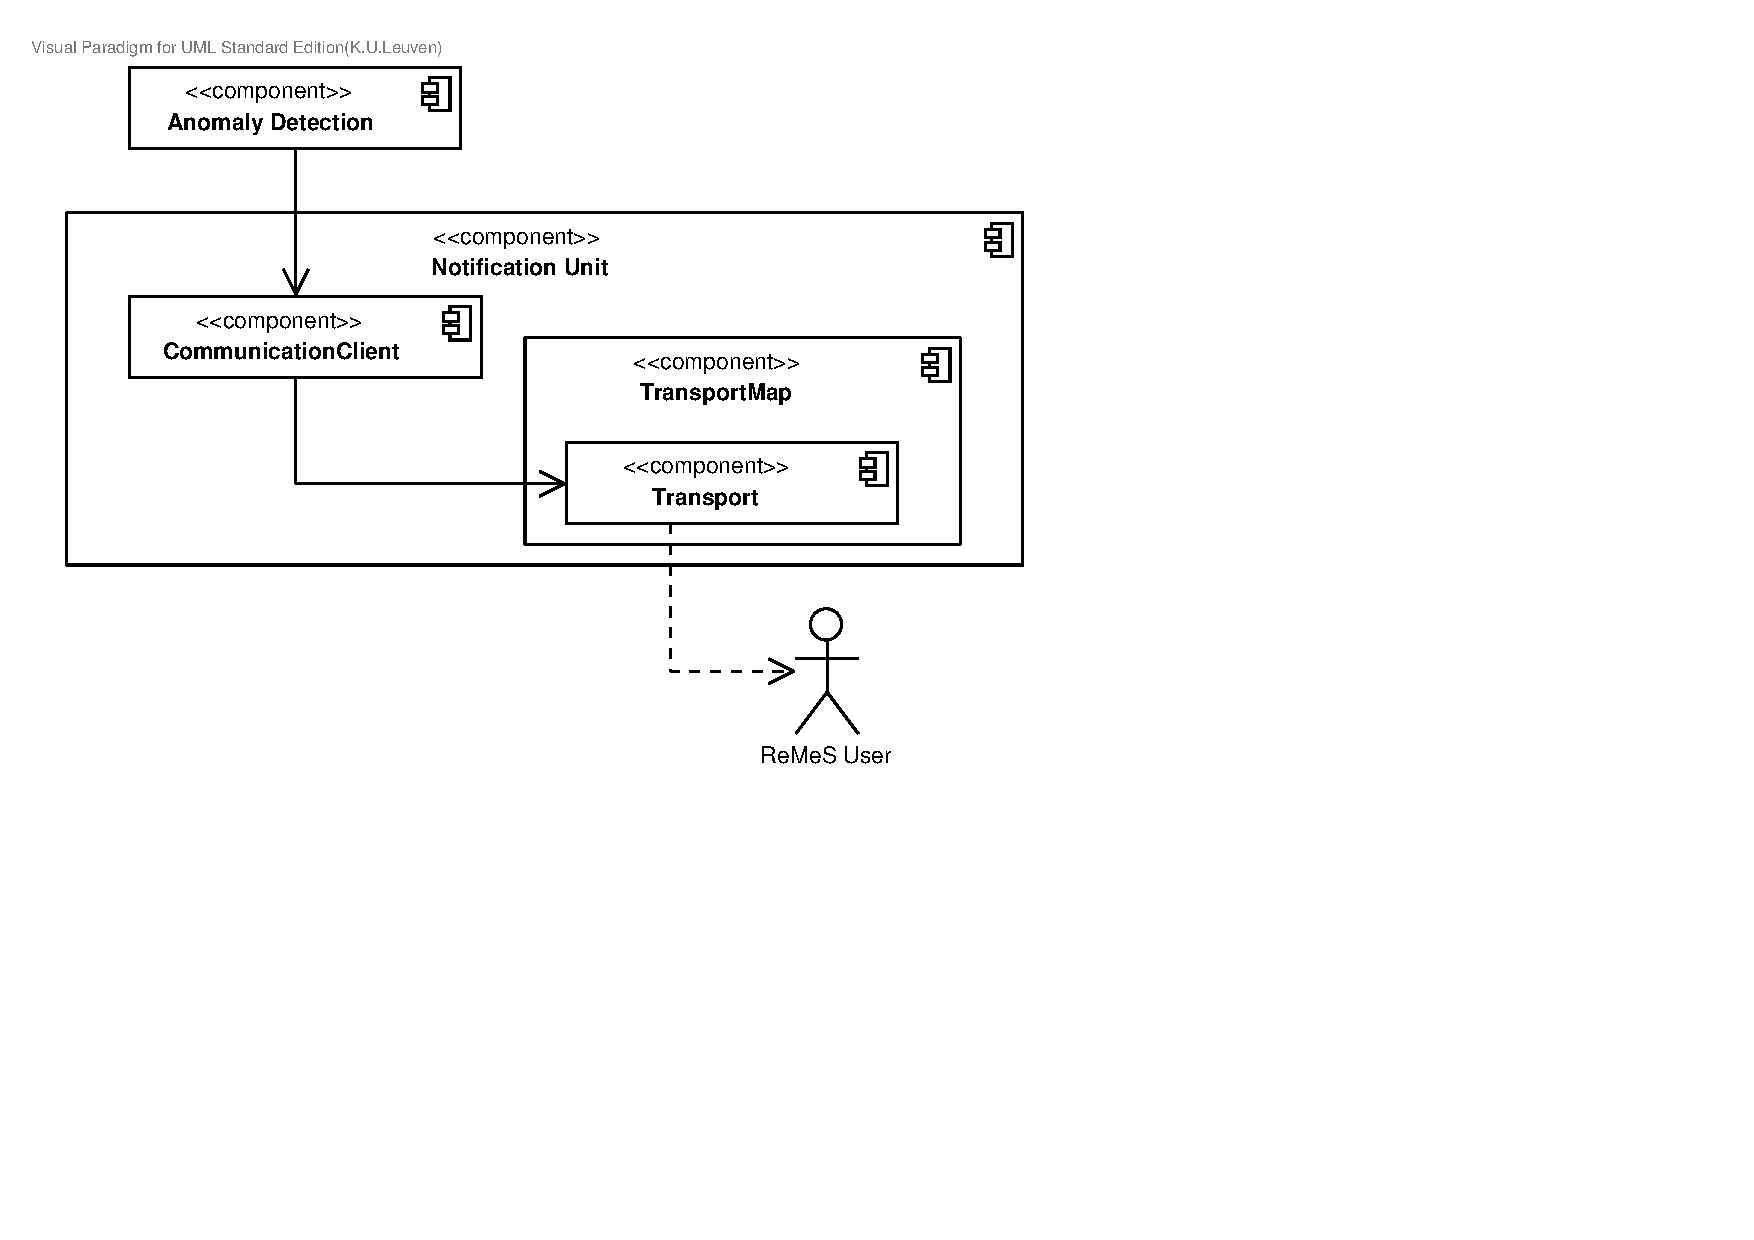
\includegraphics[width=\textwidth]{figs/add-it8-elements.pdf}
		\caption{Overview of the instantiated child elements in the Notification
		Unit.}
		\label{fig:it8/elements}
	\end{centering}
\end{figure}

\npar There are two main components in this decomposition, the
CommunicationClient and the TransportMap. Both of them will be explained below.
A graphical illustration is given in figure \ref{fig:it8/elements}.

\subsubsection{CommunicationClient} 

\npar This component gets the initial notification message. Its task is
twofold. First of all this component has to fetch the communication channel
through which it has to contact the stakeholder (i.e. the emergency services
and/or one or more customers). Therefore it uses the
\interface{RMConfigurationAPI} interface of the database which contains all user
information. Secondly, once the channel is acquired it has to contact the
TransportMap to ask for the right Transport unit which can be used to send the
notification. The TransportMap offers therefore an \interface{TransportMapAPI}
interface.

\subsubsection{Transport Map}

\npar The TransportMap is the manager of several Transport components. The
map will return the right Transport component based on the request. Each
Transportcomponent is responsible for communication towards the stakeholders
through a specific channel. To realize this, each of these Transport components
offers a \interface{TransportAPI} interface. By splitting the transport into
different components the sending of notifications can be parallelized (i.e. over
different communication channels).

\subsection{Step 4: Define interfaces for instantiated elements}
\label{add:it8/interfaces}

\npar In this section each interface is explained in terms of the components
which use and/or offer it together with information about what is exchanged. For
detailed information with reference to the specific methods the interfaces
implement, we refer to the interface catalog, see appendix
\ref{chap:interface-catalog}.

\subsubsection{NotificationAPI}

\npar The \interface{NotificationAPI} was already discussed in section
\ref{add:it1/interfaces}.

\subsubsection{TransportMapAPI}

\npar The \interface{TransportMapAPI} interface is situated in between the
CommunicationClient, which is the invoker, and TransportMap, which is the
provider. This interface offers functionality to retrieve a Transport entity.

\paragraph{TransportAPI}

\npar This interface is offered by Transport components. It is used to transport
notifications towards stakeholders such as customers.

\begin{figure}[H]
	\begin{centering}
		% TODO Figure
		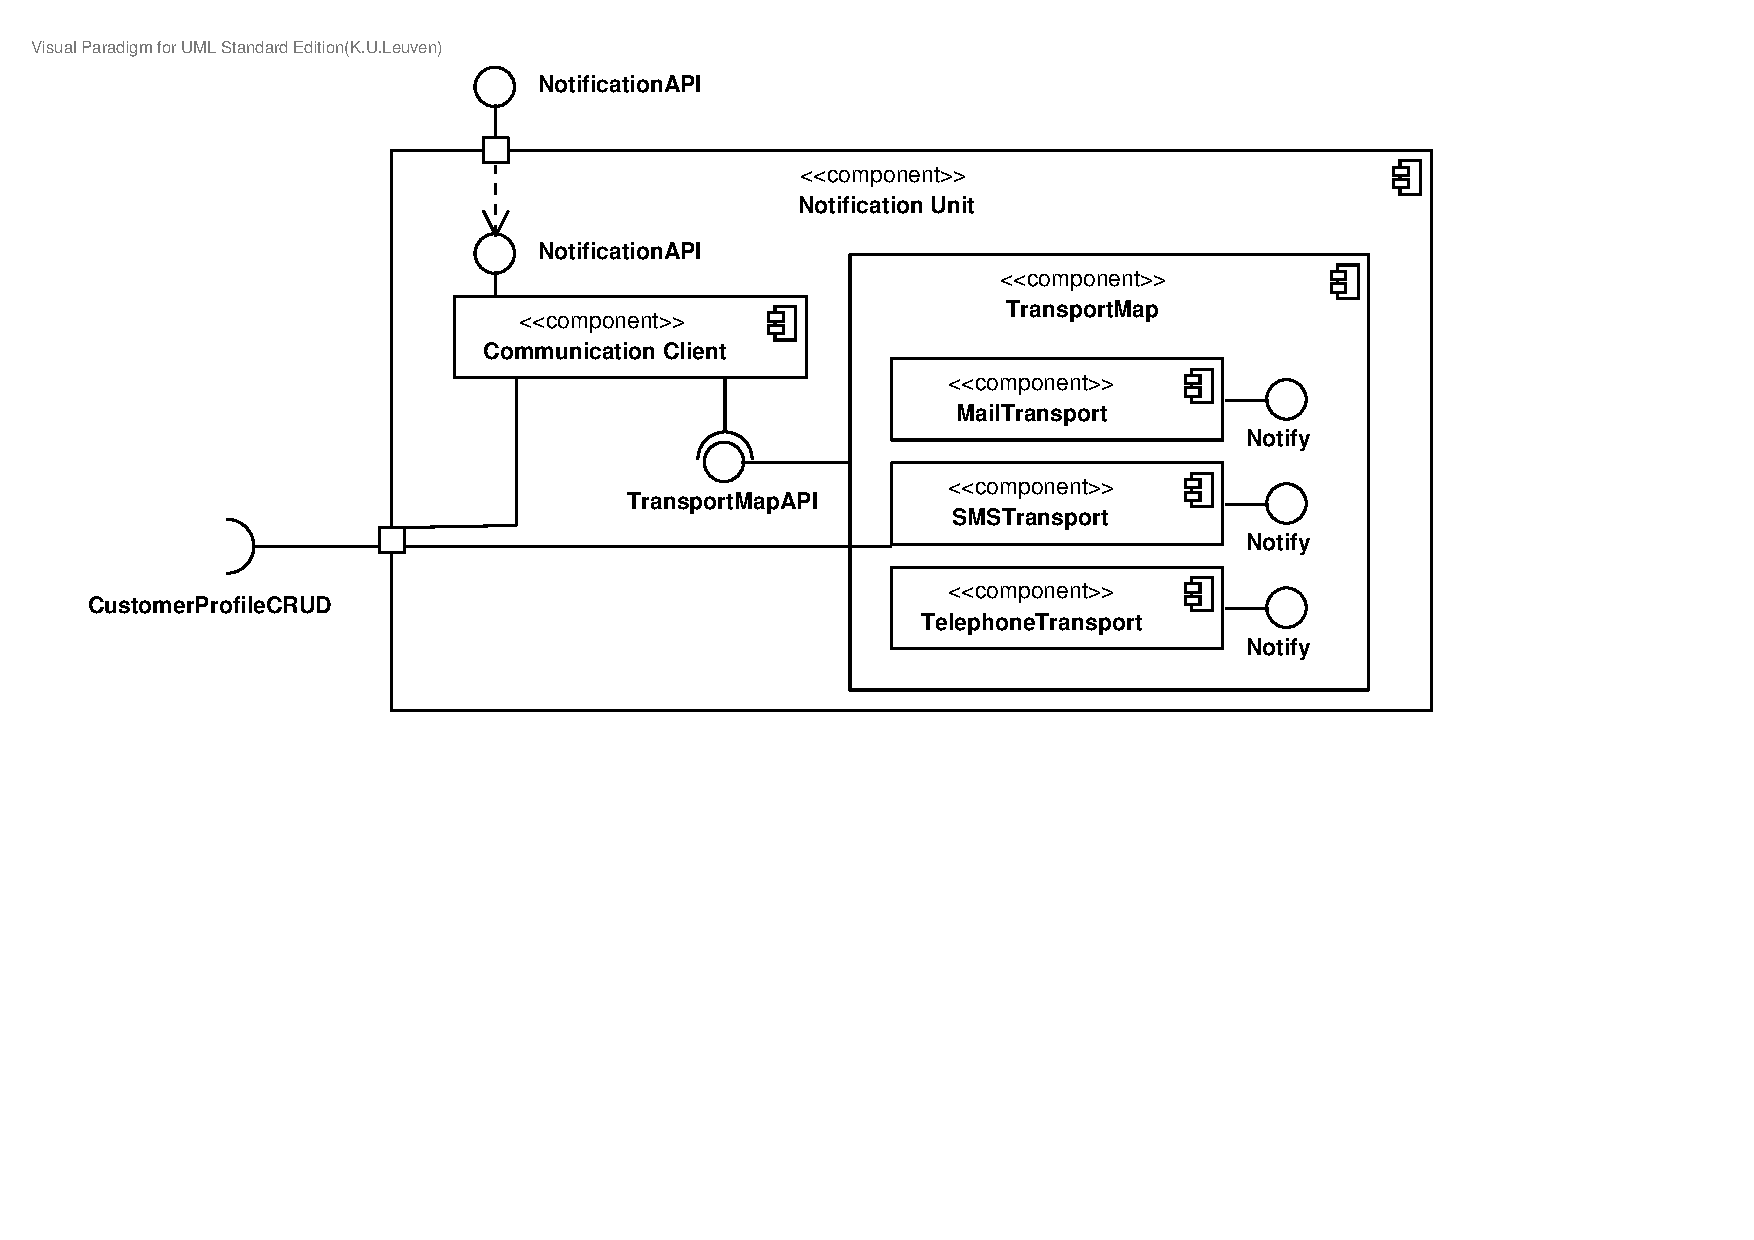
\includegraphics[width=\textwidth]{figs/add-it8-interfaces.pdf}
		\caption{Overview of the interfaces and components in the Notification Unit.}
		\label{fig:it8/interfaces}
	\end{centering}
\end{figure}

\subsection{Step 5: Verify and refine}
\label{add:it8/verification}

\npar The drivers of this iteration, UC9 and Ucx, are resolved. All the steps of
its main scenario are now tracable in the diagram.
